\label{sec:introdutction}
In recent years, with the development of the hardware and algorithms, the capabilities of a single agent have been greatly improved.
To further expand the capabilities of intelligent robots, using several robots can accelerate many tasks, such as localization, exploration, and mapping.
As simultaneous localization and mapping(SLAM) is an essential component in many tasks, it is important to do SLAM across different robots in many multi-agent applications. 
The camera is a widely used snesor in SLAM for its rich information and low cost. 
However, in many scenarios, communication is limited, so that there is no server or an agent can stably collect all of the visual data from each robot.

Therefore, to reduce communication requirements, the previous work \cite{Cieslewski:20187ee} proposes a data-efficient decentralized SLAM(DSLAM) system. 
The DSLAM frame in \cite{Cieslewski:20187ee} is illustrated in \cref{fig:all_pre}.
It makes improvements in three typical components in the DSLAM system: 1) Using ORB-SLAM \cite{orbslam} in stereo configuration as the visual odometry (VO) algorithm which provides basic intra-robot pose estimation. 2) Using NetVLAD \cite{Arandjelovic:2017997} algorithm to do place recognition which relates the current observation to previous scenes and other robots. 3) Using distributed Gauss-Seidel algorithm \cite{parallel_distributed} as the optimization back-end which optimizes the intra-robot position and fuses the inter-robot locations and maps. Each agent executes the ORB-SLAM which contains three steps for each input frame: feature extraction, feature matching and RANSAC. The NetVLAD method can encode the camera frame to a short vector which can be transformed to the server or a central agent with low communication cost.

However, both ORB-SLAM and NetVLAD require tremendous computation and storage resources, and thus, the deployment of DSLAM on embedded system is challaged by the limited resources and power supply.

% Recent advances in the deep learning and the convolution neural network (CNN) enable powerful end-to-end mode for place recognition \cite{Noh:2017d0b,Arandjelovic:2017997}, and the NetVLAD method is one of the most accurate method based on CNN. The NetVLAD algorithm based on VGG-16 model \cite{vgg16} consumes more than 80G operations for a single $300 \times 300$ input image (each operation means a addition or a multiplication). It is very challaging to deploy the NetVLAD on a tranditional embedded hardware platform.
% As to ORB-SLAM, the algorithm needs to calculate the feature point and the corresponding descriptors for each frame from camera, which is also difficult for embedded CPUs.

% With the development of FPGA, some previous work accelerate ORM-SLAM or CNN by designing specific hardware architecture. %这里需要增加一段,讲一讲ORB要多么占资源,虽然有些硬件上面的工作,但是不能同时在FPGA上既实现ORB-SLAM又实现CNN加速器。

Though NetVLAD consumes huge computation, with the development of FPGA accelerators, we use the embedded CNN accelerator on FPGA \cite{deephi} to perform NetVLAD for each frame.
We also notice that there are also some previous works regression the 6-D pose directly from the input setero camera \cite{setero2018} or monocular camera \cite{Li:2018ca8,Zhan:2018e92}, With the development of CNN.
We adopt Depth-VO-Feat \cite{Zhan:2018e92} in DSLAM system to estimate the pose from the input monocular camera.
Because Depth-VO-Feat is trained with stereo input frames and inferenced with monocular camera, the CNN method can provide absolute scale from monocular camera, and also be accelerated with our CNN accelerator. Thus we do not need to execute ORB-SLAM on embedded CPUs. 

The proposed DSLAM framework is illustrated in \cref{fig:all_us}. To make the DSLAM system more energy efficient and hardware friendly, we propose a novel hardware-software co-design DSLAM framework with the following contributions:
\begin{itemize}
\item We implement NetVLAD on an embedded SoC platform with CPU cores and FPGA fabric.
\item We use an end-to-end CNN based method to estimate the 6-DoF pose between intra-robot successive frames and matched scenes between different robots.
\item We demonstrate that our proposed hardware-software co-design decentralized SLAM system can achieve a similar accuracy with the current state-of-the-art DSLAM system without increase of communication.
\end{itemize}

\begin{figure*}[thb]
    \begin{minipage}[t]{0.5\linewidth}  
    \centering
    \subfigure[DSLAM in \cite{Cieslewski:20187ee}] {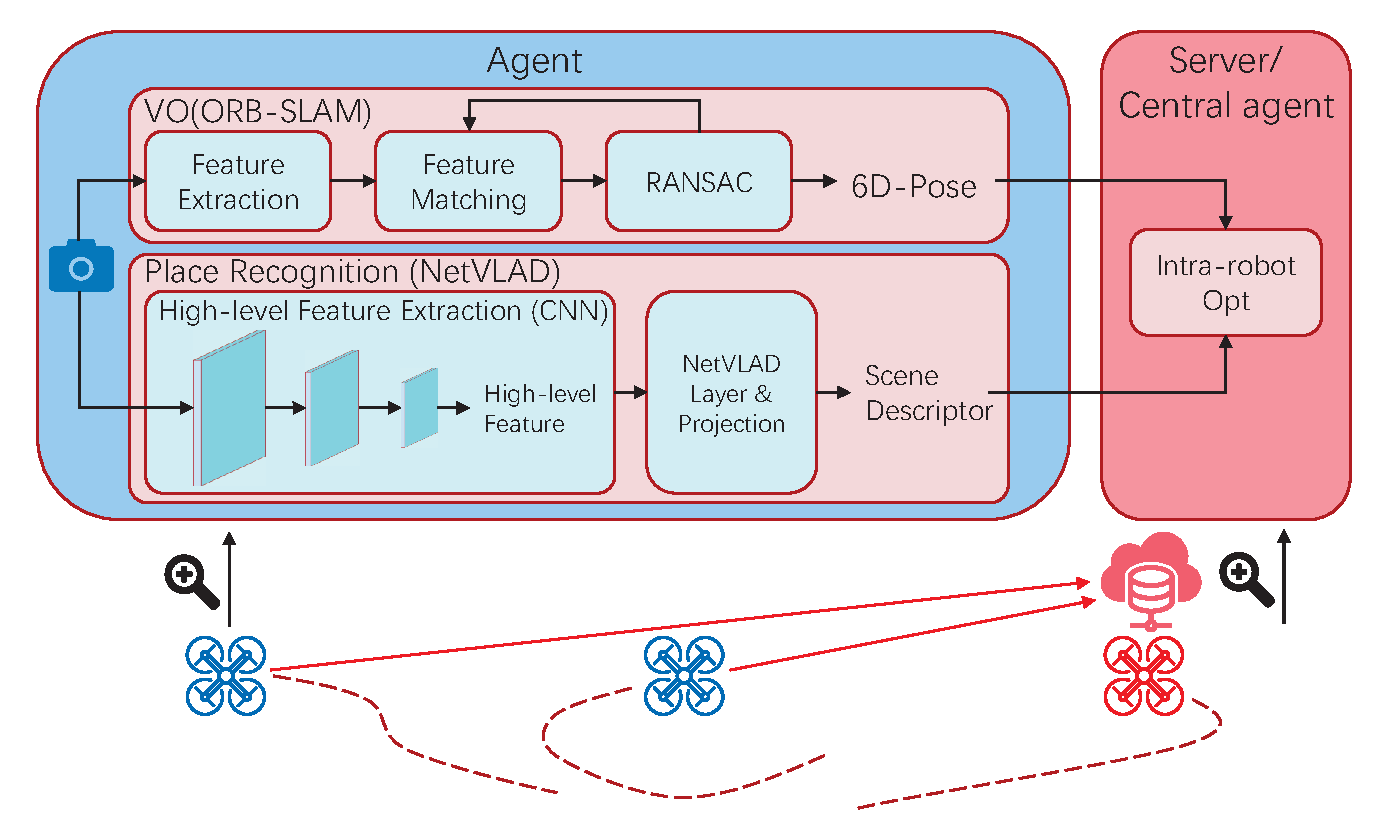
\includegraphics[width=0.95\textwidth]{fig/overview_pre.eps}\label{fig:all_pre}}
    \end{minipage}
    \begin{minipage}[t]{0.5\linewidth}  
    \centering  
    \subfigure[Our hardware-software co-design DSLAM.] {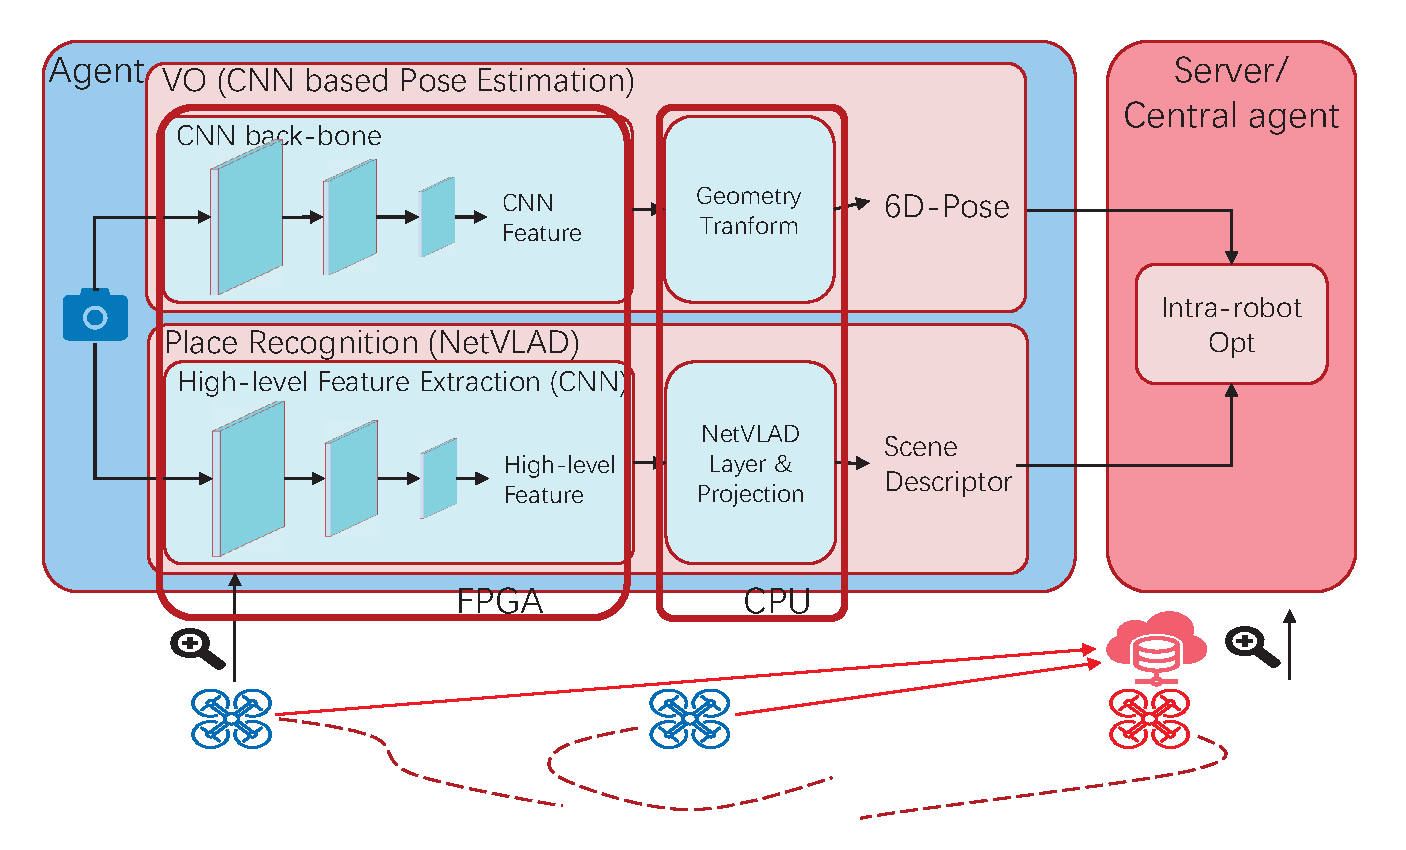
\includegraphics[width=0.95\linewidth]{fig/overview_us.eps}\label{fig:all_us}} 
    \end{minipage}
    \caption{Overview of the DSLAM in \cite{Cieslewski:20187ee} and our hardware-software co-design DSLAM. Each agent (blue drones) will send the result of 6-D pose estimation and scene descriptor to a server or a central agent (red server or drone in figure) to do inter-robot place recognition and optimization. We use CNN instead of feature points to do pose estimation so that we can use CNN accelerator to speed up the whole process.}
    \label{fig:overview}
    \end{figure*}

The rest part of this article is orgnized as follows. \Cref{sec:background} will give the basic idea of CNN based methods and the hardware architecture of embedded FPGA. \Cref{sec:hardsoft} will detail the implementation of our hardware-software co-design DSLAM system. The experiment result will be given in \Cref{sec:experiment}. \Cref{sec:conclusion} will conclude this paper.